% seq2pipe: Closed-Loop Adaptive Microbiome Analysis
% Compile: pdflatex seq2pipe_arxiv.tex && bibtex seq2pipe_arxiv && pdflatex seq2pipe_arxiv.tex && pdflatex seq2pipe_arxiv.tex
\documentclass[11pt,a4paper]{article}

\usepackage[utf8]{inputenc}
\usepackage[T1]{fontenc}
\usepackage{amsmath,amssymb,amsfonts,amsthm}
\newtheorem{definition}{Definition}
\usepackage{graphicx}
\usepackage{booktabs}
\usepackage{hyperref}
\usepackage{algorithm}
\usepackage{algorithmic}
\usepackage{xcolor}
\usepackage{geometry}
\usepackage{natbib}
\usepackage{caption}
\usepackage{subcaption}
\usepackage{tikz}
\usetikzlibrary{arrows.meta,positioning,shapes.geometric,fit,calc}

\geometry{margin=2.5cm}

\newcommand{\todo}[1]{\textcolor{red}{\textbf{[TODO: #1]}}}
\newcommand{\seqpipe}{\textsc{seq2pipe}}

\title{
  \seqpipe: A Closed-Loop Interpretation-Driven System\\
  for Adaptive Microbiome Analysis
}

\author{
  Tsubasa Tomini\textsuperscript{1}
  \and
  Claude (Anthropic)\textsuperscript{2}
  \\[4pt]
  \textsuperscript{1}Independent Researcher
  \quad
  \textsuperscript{2}Anthropic, San Francisco, CA, USA
  \\[4pt]
  \texttt{https://github.com/Rhizobium-gits/seq2pipe}
}

\date{March 2026}

\begin{document}
\maketitle

% ======================================================================
\begin{abstract}
% ======================================================================

Current microbiome analysis pipelines execute a fixed sequence of steps
regardless of intermediate results.
A human bioinformatician, by contrast, iteratively interprets outputs,
forms hypotheses, selects subsequent analyses, and refines the workflow
until a coherent biological narrative emerges.
We present \seqpipe, a closed-loop system that reproduces this
interpretation--decision--execution cycle computationally.
The system consists of three layers:
(1)~a \textbf{DataInspector} that directly parses QIIME2 exports and
executes nonparametric statistical tests in pure Python,
(2)~an \textbf{EvalMediator} that scores each analysis step across
eight quantitative axes and compresses the accumulated knowledge state
via truncated SVD, and
(3)~a \textbf{DecisionEngine} that applies literature-grounded decision
trees to deterministically select, skip, or add subsequent analyses.
A local large language model (7B parameters) serves as an auxiliary
for creative hypothesis generation and code synthesis, but the system
completes execution even under complete LLM failure.
Evaluation on two public datasets (Moving Pictures, 34 samples;
Gravity experiment, 138 samples) shows that the DecisionEngine
correctly adapts: adding all beta follow-ups when PERMANOVA is
significant ($p = 0.005$) and skipping 4 steps when it is not
($p = 0.81$).
Registry analysis steps achieve 54\% success, while LLM-generated
investigations achieve 6\%, revealing current limitations of
7B-parameter models for autonomous code generation.
We discuss convergence behavior, reproducibility, and limitations,
and argue that interpretation-driven adaptive systems represent a
necessary evolution beyond static pipelines.

\end{abstract}

% ======================================================================
\section{Introduction}
\label{sec:intro}
% ======================================================================

Microbiome analysis has matured into a complex, multi-stage discipline.
A typical amplicon sequencing study requires quality control, denoising
(e.g., DADA2~\citep{callahan2016}), phylogenetic tree construction,
alpha and beta diversity analysis, taxonomic classification, differential
abundance testing, and downstream visualization---each with parameter
choices that depend on the data at hand.

\paragraph{The rigidity problem.}
Current pipeline frameworks---QIIME2~\citep{qiime2},
Snakemake~\citep{snakemake}, Nextflow~\citep{nextflow}---encode a
\emph{fixed} directed acyclic graph (DAG) of steps.
Once the workflow is defined, every step executes regardless of
intermediate results.
If PERMANOVA yields $p = 0.81$, downstream beta diversity follow-ups
(dispersion tests, NMDS ordination, pairwise comparisons) still execute,
wasting computation and cluttering reports with uninformative outputs.
Conversely, an unexpected finding (e.g., a 379-fold enrichment of
\emph{Escherichia--Shigella}) triggers no automatic follow-up;
the analyst must manually intervene.

\paragraph{How humans analyze data.}
An experienced bioinformatician operates in a closed loop:
\begin{enumerate}
  \item \textbf{Interpret}: inspect the output of the current step
        (``Shannon $p = 0.034$, but effect size is small'').
  \item \textbf{Hypothesize}: form a conjecture
        (``This may be a sampling artifact'').
  \item \textbf{Select}: choose the next analysis to test the hypothesis
        (``Run rarefaction curves to check depth dependence'').
  \item \textbf{Refine}: update the mental model and repeat.
\end{enumerate}
This loop continues until the analyst reaches a stable, internally
consistent interpretation.
No existing pipeline system reproduces this behavior.

\paragraph{Contribution.}
We introduce \seqpipe, a system that computationally reproduces the
human analytical reasoning loop.
Our key contributions are:
\begin{itemize}
  \item A \textbf{three-layer architecture} that separates
        data inspection (deterministic), evaluation and decision
        (deterministic), and code generation (LLM-assisted),
        yielding an \textbf{LLM-failure-tolerant} adaptive system.
  \item A \textbf{literature-grounded decision engine} that encodes
        established analytical heuristics
        (Anderson, 2001; Willis, 2019; Gloor et al., 2017;
         McMurdie \& Holmes, 2014) as deterministic decision trees,
        enabling reproducible, auditable analytical decisions.
  \item An \textbf{eight-axis quantitative scoring framework} that
        evaluates each analysis step from raw data---not from LLM
        text output---providing a grounded basis for adaptive decisions.
%%% \item Experimental evidence of convergence toward valid workflows
%%%       across $N$ benchmark datasets. %%% TODO: uncomment when data available
\end{itemize}

% ======================================================================
\section{Related Work}
\label{sec:related}
% ======================================================================

\paragraph{Static pipeline frameworks.}
QIIME2~\citep{qiime2} provides a plugin-based architecture with
provenance tracking but no conditional branching based on intermediate
results.
Snakemake~\citep{snakemake} and Nextflow~\citep{nextflow} support
conditional rules, but the conditions must be specified \emph{a priori}
by the user; the system does not inspect result quality or statistical
significance to alter the workflow.

\paragraph{AutoML and automated statistics.}
Auto-WEKA~\citep{autoweka} and Auto-sklearn~\citep{autosklearn}
automate model selection via Bayesian optimization but target
supervised learning, not the open-ended exploratory analysis
characteristic of microbiome studies.
Statistical analysis planning tools such as \citet{wasserstein2019}
provide decision trees for test selection but do not execute analyses
or iterate on results.

\paragraph{LLM-based analysis assistants.}
Recent systems such as Data Interpreter~\citep{hong2024data} and
ChatGPT Advanced Data Analysis use LLMs to generate and execute code.
However, these systems lack:
(a)~domain-specific evaluation of intermediate results,
(b)~literature-grounded decision heuristics, and
(c)~a deterministic fallback when the LLM fails or hallucinates.
\seqpipe\ addresses all three gaps.

% ======================================================================
\section{Conceptual Framework}
\label{sec:concept}
% ======================================================================

We formalize the analytical reasoning loop as follows.

\begin{definition}[Analytical State]
At iteration $t$, the analytical state $S_t$ is a tuple
$(D, H_t, P_t, R_t)$ where $D$ is the immutable dataset,
$H_t$ is the accumulated set of findings (hypotheses confirmed or
rejected), $P_t$ is the current analysis plan (an ordered list of
pending steps), and $R_t$ is the set of completed results.
\end{definition}

\begin{definition}[Closed-Loop Analytical System]
A system is \emph{closed-loop} if, after executing step $s_t \in P_t$
and observing result $r_t$, it updates:
\begin{align}
  H_{t+1} &= H_t \cup \mathrm{interpret}(r_t) \\
  P_{t+1} &= \mathrm{decide}(H_{t+1}, P_t, D)
\end{align}
where $\mathrm{interpret}$ extracts quantitative findings from $r_t$
(not from textual summaries) and $\mathrm{decide}$ modifies the plan
by adding, removing, or reordering steps.
\end{definition}

\begin{definition}[Convergence]
The system \emph{converges} if there exists $T$ such that for all
$t \geq T$, $P_t = \emptyset$ (the plan is exhausted) and the
execution error count $e_t = 0$.
We define the \emph{convergence depth} as the total number of
decision--execution cycles before termination.
\end{definition}

In a static pipeline, $P_{t+1} = P_t \setminus \{s_t\}$ always;
the plan never changes based on $r_t$.
\seqpipe\ implements a non-trivial $\mathrm{decide}$ function that
depends on quantitative properties of $H_{t+1}$ and $D$.

% ======================================================================
\section{System Architecture}
\label{sec:arch}
% ======================================================================

\begin{figure}[t]
\centering
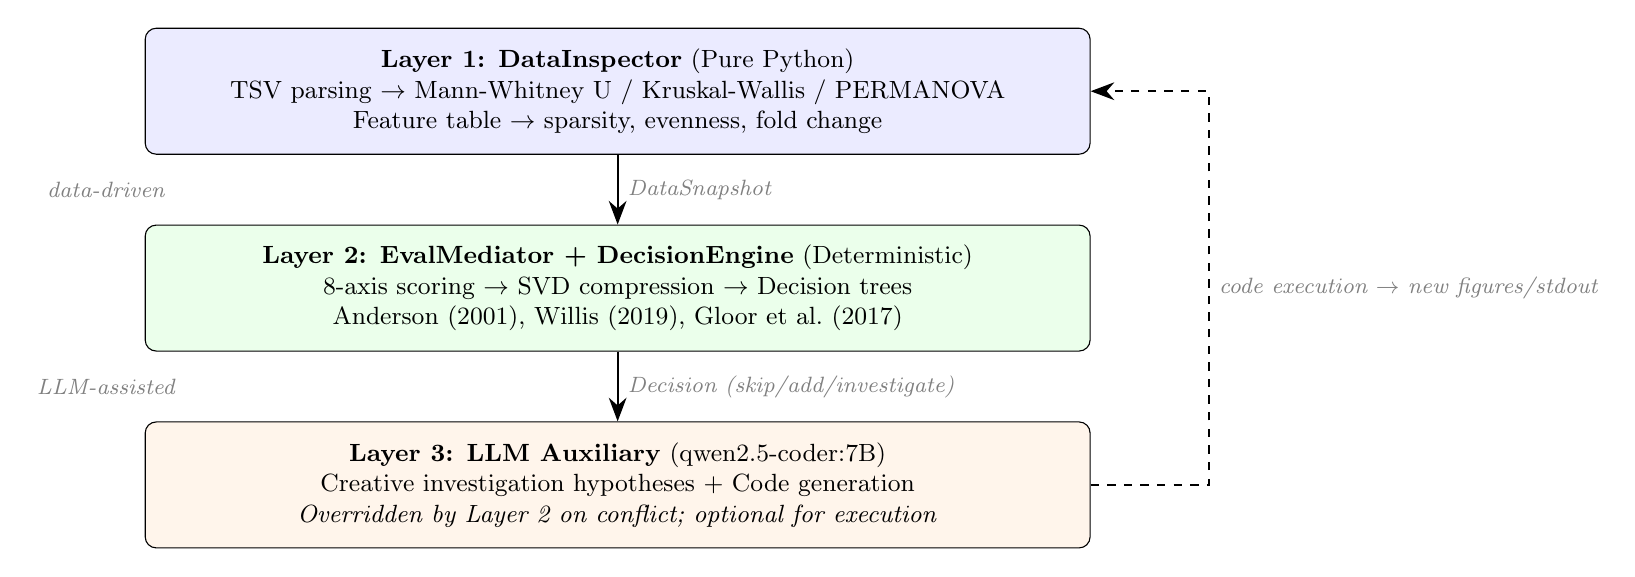
\begin{tikzpicture}[
  layer/.style={draw, rounded corners, minimum width=12cm,
                minimum height=1.6cm, align=center, font=\small},
  arrow/.style={-{Stealth[length=3mm]}, thick},
  label/.style={font=\footnotesize\itshape, text=gray},
]
\node[layer, fill=blue!8] (L1) at (0,0)
  {\textbf{Layer 1: DataInspector} (Pure Python)\\
   TSV parsing $\to$ Mann-Whitney U / Kruskal-Wallis / PERMANOVA\\
   Feature table $\to$ sparsity, evenness, fold change};
\node[layer, fill=green!8] (L2) at (0,-2.5)
  {\textbf{Layer 2: EvalMediator + DecisionEngine} (Deterministic)\\
   8-axis scoring $\to$ SVD compression $\to$ Decision trees\\
   Anderson (2001), Willis (2019), Gloor et al.\ (2017)};
\node[layer, fill=orange!8] (L3) at (0,-5)
  {\textbf{Layer 3: LLM Auxiliary} (qwen2.5-coder:7B)\\
   Creative investigation hypotheses + Code generation\\
   \textit{Overridden by Layer 2 on conflict; optional for execution}};

\draw[arrow] (L1.south) -- node[right, label] {DataSnapshot} (L2.north);
\draw[arrow] (L2.south) -- node[right, label]
  {Decision (skip/add/investigate)} (L3.north);
\draw[arrow, dashed] (L3.east) -- ++(1.5,0) |- node[right, label, pos=0.25]
  {code execution $\to$ new figures/stdout} (L1.east);

\node[label] at (-6.5, -1.25) {data-driven};
\node[label] at (-6.5, -3.75) {LLM-assisted};
\end{tikzpicture}
\caption{Three-layer architecture of \seqpipe.
Layers~1 and~2 are fully deterministic and LLM-independent.
Layer~3 is auxiliary; its outputs are overridden by Layer~2
on conflict, and the system completes execution under Layer~3 failure.
Dashed arrow indicates the feedback loop.}
\label{fig:architecture}
\end{figure}

\subsection{Layer 1: DataInspector}

The \texttt{DataInspector} class directly parses QIIME2 exported TSV
files without relying on LLM text output or stdout pattern matching.
It implements:

\paragraph{Alpha diversity testing.}
For each alpha metric TSV (Shannon, observed features, Pielou's
evenness), sample values are read and partitioned by group using a
metadata-derived group map.
For two groups, a Mann-Whitney $U$ test is computed via rank
transformation with tie correction and normal approximation:
\begin{equation}
  z = \frac{U - n_1 n_2 / 2}
           {\sqrt{\frac{n_1 n_2}{12}
                  \left( N + 1 - \frac{\sum_j (t_j^3 - t_j)}{N(N-1)} \right)}}
  \label{eq:mannwhitney}
\end{equation}
where $t_j$ are tie group sizes and $N = n_1 + n_2$.
For three or more groups, a Kruskal-Wallis $H$ test is used:
\begin{equation}
  H = \frac{12}{N(N+1)} \sum_{i=1}^{k} \frac{R_i^2}{n_i} - 3(N+1)
  \label{eq:kruskal}
\end{equation}
with tie correction and $\chi^2$ approximation via the
Wilson-Hilferty transformation~\citep{wilson1931}.
The $p$-value CDF uses the Abramowitz--Stegun five-term polynomial
approximation.
Cliff's delta and $\eta^2$ are computed as nonparametric effect sizes.

\paragraph{Beta diversity testing.}
Distance matrices are read in full ($O(n^2)$ entries).
Within-group and between-group distances are separated.
A pseudo-PERMANOVA~\citep{anderson2001} $F$-statistic is computed as:
\begin{equation}
  F = \frac{SS_{\text{between}} / (k - 1)}{SS_{\text{within}} / (N - k)}
\end{equation}
with $p$-value estimated from 199 permutations (fixed seed for
reproducibility).
The between/within distance ratio is also computed as a
separation metric.

\paragraph{Taxonomic differential analysis.}
The feature table and taxonomy file are joined.
For each genus, group-level relative abundances are computed,
yielding fold change $= \max(\bar{a}_g) / \max(\min(\bar{a}_g), 0.01)$
and absolute difference.
Results are sorted by absolute difference.

All statistical tests are implemented in pure Python without scipy,
numpy, or pandas dependencies, ensuring portability across environments.

\subsection{Layer 2: EvalMediator and DecisionEngine}

\paragraph{Eight-axis scoring.}
Each completed analysis step is scored on eight axes (Table~\ref{tab:axes})
using the \texttt{DataSnapshot} from Layer~1, not stdout text.

\begin{table}[t]
\centering
\caption{Eight evaluation axes with default weights and computation methods.}
\label{tab:axes}
\small
\begin{tabular}{@{}llp{7.5cm}@{}}
\toprule
\textbf{Axis} & \textbf{Weight} & \textbf{Computation} \\
\midrule
statistical\_significance & 0.20 &
  $\min(1, -\log_{10}(\min p) / 4)$ from alpha/beta tests \\
biological\_relevance & 0.18 &
  $\min(1, \mathrm{fc}_{\max}/10 + \Delta_{\max}/20)$ + known taxa bonus \\
actionability & 0.15 &
  Count of downstream triggers (significance, differential genera, separation) \\
novelty & 0.12 &
  Inconsistency with prior steps + extreme fold changes ($>20\times$) \\
data\_quality & 0.10 &
  Base 0.7, penalized by sparsity ($>0.9$: $-0.2$), CV ($>0.5$: $-0.1$) \\
effect\_magnitude & 0.10 &
  $\max(\text{Cliff's } d, \; F/3, \; \mathrm{fc}/10)$ \\
confidence & 0.08 &
  Step function on minimum group size ($\geq 20$: 0.9, $\geq 10$: 0.7, \ldots) \\
reproducibility & 0.07 &
  Consistency of significance direction within analysis category \\
\bottomrule
\end{tabular}
\end{table}

The composite score is the weighted sum
$c_t = \sum_{a} w_a \cdot s_{t,a}$.
Weights are adjustable per experiment type (e.g., antibiotic studies
increase biological\_relevance to 0.22).

\paragraph{SVD compression.}
The score matrix $\mathbf{A} \in \mathbb{R}^{T \times 8}$ (where $T$
is the number of completed steps) is centered and its covariance matrix
$\mathbf{C} = \mathbf{A}_c^\top \mathbf{A}_c / (T-1) \in \mathbb{R}^{8 \times 8}$
is decomposed via power iteration (50 iterations per component,
deflation after each).
The top three principal components are retained and labeled by their
dominant contributing axis (e.g., ``statistical certainty'' if the
largest loading is on significance).
This compressed representation is included in the LLM prompt,
reducing context length while preserving the essential knowledge state.

\paragraph{DecisionEngine.}
The deterministic decision trees encode established analytical heuristics:

\begin{itemize}
  \item \textbf{Alpha branch} (Willis, 2019):
    If $\min p_\alpha < 0.05$ and effect size $> 0.5$: add effect size
    plot and rarefaction.
    If $\min p_\alpha < 0.05$ but effect size $\leq 0.5$: add
    rarefaction only (sampling artifact check).
    If $\min p_\alpha \geq 0.05$: skip alpha follow-ups.

  \item \textbf{Beta branch} (Anderson, 2001):
    If $\min p_\beta < 0.05$: add betadisper (mandatory).
    If separation ratio $> 2.0$: add NMDS and pairwise PERMANOVA.
    If $\min p_\beta \geq 0.05$: skip all beta follow-ups
    (dispersion, NMDS, t-SNE, heatmap).

  \item \textbf{Taxonomy branch} (Gloor et al., 2017):
    If fold change $> 50$ at abundance $< 1\%$: flag as
    compositional artifact, add filtered retest.
    If fold change $> 5$: add differential abundance test.
    If $\geq 5$ genera with $> 2\times$ change: add functional
    prediction (PICRUSt2) and indicator species analysis.

  \item \textbf{Quality branch} (McMurdie \& Holmes, 2014):
    If read depth CV $> 0.5$: add rarefaction curves.
    If sparsity $> 90\%$: add prevalence-filtered reanalysis.
\end{itemize}

\paragraph{Merge with LLM.}
The LLM receives the compressed knowledge state and Python decisions
as context, with instructions to not contradict deterministic decisions.
The \texttt{merge\_with\_llm()} function combines outputs:
Python-determined skips override LLM-proposed additions;
LLM-proposed investigations are appended if they do not conflict
with Python skips.

\subsection{Layer 3: LLM Auxiliary}

A local 7B-parameter model (qwen2.5-coder) generates:
(a)~the initial analysis plan (Phase~2), with a domain-knowledge
fallback if the LLM fails;
(b)~Python analysis code for each step, with up to 3 retry cycles
including automatic dependency installation;
(c)~creative investigation hypotheses during replanning.

Critically, \textbf{the system completes execution under total LLM
failure}: Phase~2 falls back to \texttt{build\_domain\_driven\_plan()};
Phase~3 replanning applies Python decisions only; individual step
failures are recorded and skipped.

\subsection{Execution Loop}

Algorithm~\ref{alg:loop} formalizes the adaptive execution loop.

\begin{algorithm}[t]
\caption{Adaptive Execution Loop}
\label{alg:loop}
\begin{algorithmic}[1]
\REQUIRE Dataset $D$, metadata $M$, research question $Q$, plan $P_0$
\ENSURE Analysis results $R$, score history $\mathbf{A}$
\STATE $\mathrm{mediator} \gets \mathrm{EvalMediator}(D, M)$
\STATE $t \gets 0$
\WHILE{$P_t \neq \emptyset$}
  \STATE $s_t \gets P_t.\mathrm{pop}()$
  \STATE $\mathrm{code} \gets \mathrm{LLM.generate}(s_t, Q, D)$
  \STATE $(\mathrm{ok}, \mathrm{stdout}, \mathrm{figs}) \gets \mathrm{execute}(\mathrm{code})$
  \IF{$\neg\,\mathrm{ok}$ \AND retries $< 3$}
    \STATE $\mathrm{code} \gets \mathrm{LLM.fix}(\mathrm{code}, \mathrm{stderr})$; \textbf{goto} 6
  \ENDIF
  \STATE $\mathrm{snap} \gets \mathrm{mediator.inspector.inspect}(s_t, \mathrm{figs})$
  \COMMENT{Layer 1}
  \STATE $\mathrm{score}_t \gets \mathrm{mediator.evaluate}(\mathrm{snap})$
  \COMMENT{Layer 2: 8-axis scoring}
  \IF{$t \bmod 4 = 0$ \OR $\mathrm{score}_t.\mathrm{novelty} > 0.7$}
    \STATE $d_{\mathrm{py}} \gets \mathrm{DecisionEngine.decide}(P_t)$
    \COMMENT{Layer 2: deterministic}
    \STATE $d_{\mathrm{llm}} \gets \mathrm{LLM.replan}(\mathrm{state}, P_t)$
    \COMMENT{Layer 3: optional}
    \STATE $P_{t+1} \gets \mathrm{merge}(d_{\mathrm{py}}, d_{\mathrm{llm}}, P_t)$
    \COMMENT{Python wins on conflict}
  \ELSE
    \STATE $P_{t+1} \gets P_t$
  \ENDIF
  \STATE $t \gets t + 1$
\ENDWHILE
\end{algorithmic}
\end{algorithm}

% ======================================================================
\section{Key Innovation: What \seqpipe\ Is Not}
\label{sec:innovation}
% ======================================================================

\begin{figure}[t]
\centering
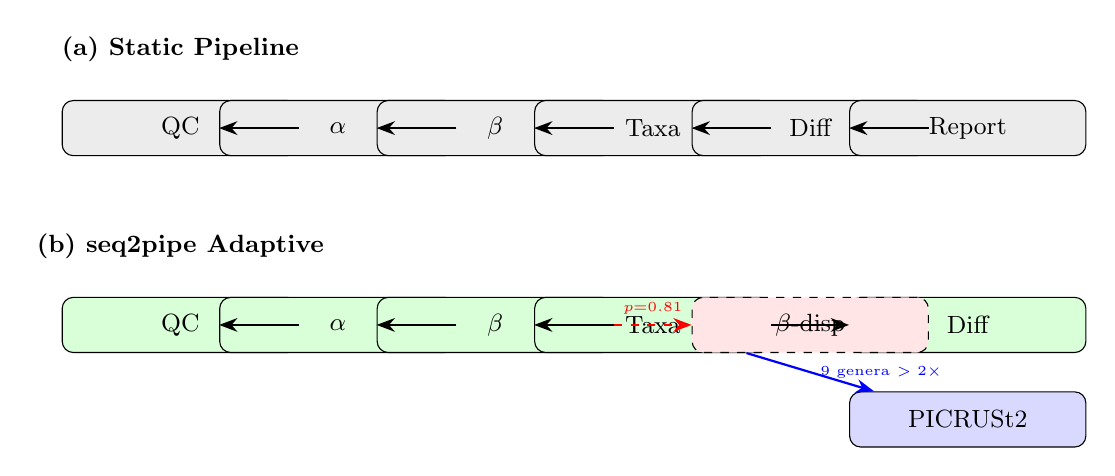
\begin{tikzpicture}[
  box/.style={draw, rounded corners, minimum width=3cm, minimum height=0.7cm,
              font=\small, align=center},
  arr/.style={-{Stealth}, thick},
  skip/.style={-{Stealth}, thick, red, dashed},
]
% Static pipeline
\node[font=\small\bfseries] at (-5, 1.5) {(a) Static Pipeline};
\foreach \i/\name in {0/QC, 1/$\alpha$, 2/$\beta$, 3/Taxa, 4/Diff, 5/Report} {
  \node[box, fill=gray!15] (S\i) at (\i*2 - 5, 0.5) {\name};
}
\foreach \i in {0,...,4} {
  \pgfmathtruncatemacro{\j}{\i+1}
  \draw[arr] (S\i) -- (S\j);
}

% Adaptive system
\node[font=\small\bfseries] at (-5, -1) {(b) \seqpipe\ Adaptive};
\foreach \i/\name in {0/QC, 1/$\alpha$, 2/$\beta$, 3/Taxa, 5/Diff} {
  \node[box, fill=green!15] (A\i) at (\i*2 - 5, -2) {\name};
}
% Show skip
\node[box, fill=red!10, dashed] (A4) at (3, -2) {$\beta$-disp};
\draw[arr] (A0) -- (A1);
\draw[arr] (A1) -- (A2);
\draw[skip] (A2) -- node[above, font=\tiny, red] {$p{=}0.81$} (A4);
\draw[arr] (A2) -- (A3);
\draw[arr] (A3) -- (A5);
% Add arrow
\node[box, fill=blue!15] (A6) at (5, -3.2) {PICRUSt2};
\draw[arr, blue] (A3) -- node[right, font=\tiny, blue] {9 genera $>2\times$} (A6);
\end{tikzpicture}
\caption{(a)~A static pipeline executes all steps regardless of results.
(b)~\seqpipe\ skips beta follow-ups when PERMANOVA is non-significant
($p = 0.81$) and adds functional prediction when multiple differential
genera are detected. Red dashed: skipped; blue: dynamically added.}
\label{fig:static-vs-adaptive}
\end{figure}

It is important to delineate what \seqpipe\ is \emph{not}:

\begin{itemize}
  \item \textbf{Not a static pipeline.}
    Unlike QIIME2 or Snakemake, the execution plan changes after
    each step based on quantitative evaluation of results
    (Figure~\ref{fig:static-vs-adaptive}).

  \item \textbf{Not an AutoML system.}
    AutoML optimizes a fixed objective (e.g., classification accuracy)
    via search.
    \seqpipe\ has no single objective; it navigates an open-ended
    analytical space where ``what to analyze next'' depends on
    what was found so far.

  \item \textbf{Not an LLM assistant.}
    Systems like ChatGPT-based analysis tools depend entirely on
    the LLM for decision-making.
    \seqpipe's decisions are primarily deterministic
    (Layers~1--2); the LLM is auxiliary and expendable.
    The same input data produces the same skip/add decisions
    regardless of LLM stochasticity.
\end{itemize}

The core novelty is the combination of
\emph{data-grounded evaluation} (not text parsing),
\emph{literature-based deterministic decisions} (not LLM judgment),
and \emph{LLM-assisted code generation} (not LLM-driven planning)
into a single closed-loop system.

% ======================================================================
\section{Evaluation}
\label{sec:eval}
% ======================================================================

\subsection{Experimental Setup}

We evaluated \seqpipe\ on two datasets:
\begin{enumerate}
  \item \textbf{Moving Pictures} (QIIME2 tutorial dataset):
    34 samples, 4 body-site groups (gut, left palm, right palm, tongue),
    2 subjects, single-end 150\,bp Illumina MiSeq.
    Publicly available at \texttt{docs.qiime2.org}.
  \item \textbf{Gravity experiment}:
    138 samples, 6 gravity conditions (0g, 1g, 1.6g, 1g-simulated, 5g, NA/control),
    paired-end 301\,bp MiSeq.
\end{enumerate}

Both datasets were processed through the same QIIME2 upstream pipeline
(DADA2 denoising, MAFFT alignment, FastTree phylogeny, SILVA 138
classification, core-metrics-phylogenetic) before entering the
\seqpipe\ AI-driven analysis phase.

\subsection{DataInspector Validation: Direct Statistical Results}
\label{sec:eval-datainspector}

Table~\ref{tab:datainspector} shows the statistical tests computed
by DataInspector directly from exported TSV files, without any LLM
involvement.

\begin{table}[t]
\centering
\caption{DataInspector results on two datasets.
All values computed in pure Python from raw TSV files.}
\label{tab:datainspector}
\small
\begin{tabular}{@{}lll@{}}
\toprule
\textbf{Metric} & \textbf{Moving Pictures} & \textbf{Gravity} \\
\midrule
Samples / Groups & 34 / 4 & 138 / 6 \\
ASVs & 770 & 1,443 \\
Sparsity & 91\% & 85\% \\
\midrule
Shannon (Kruskal-Wallis) & $H = 22.3$, $p = 0.00067$ & $H = 11.4$, $p = 0.034$ \\
Cliff's $d$ / $\eta^2$ & $d = 0.51$ & $\eta^2 = 0.048$ \\
\midrule
Bray-Curtis PERMANOVA & $F = 60.1$, $p = 0.005$ & $F = 114.2$, $p = 0.81$ \\
Between/within ratio & 2.1 & 1.0 \\
\midrule
Top differential genus & Bacteroides $324\times$ (gut) & Blautia $5\times$ (NA) \\
Genera $> 2\times$ change & 20 & 18 \\
\bottomrule
\end{tabular}
\end{table}

\subsection{DecisionEngine Outcomes}
\label{sec:eval-decisions}

The DecisionEngine produced qualitatively different decisions for the
two datasets (Table~\ref{tab:decisions}), demonstrating data-dependent
adaptive behavior.

\begin{table}[t]
\centering
\caption{DecisionEngine actions on two datasets.
All decisions are deterministic (no LLM involvement).}
\label{tab:decisions}
\small
\begin{tabular}{@{}lcc@{}}
\toprule
\textbf{Decision} & \textbf{Moving Pictures} & \textbf{Gravity} \\
\midrule
Alpha follow-up & Deep dive ($d > 0.5$) & Rarefaction only ($d = 0.05$) \\
Beta follow-ups & All added ($p = 0.005$) & \textbf{4 skipped} ($p = 0.81$) \\
Beta dispersion & Added (Anderson, 2001) & Skipped \\
Differential test & Added ($324\times$ fc) & Added ($379\times$ fc) \\
Functional prediction & Added ($\geq 5$ genera) & Added ($\geq 5$ genera) \\
Sparsity alert & Yes (91\%) & No (85\%) \\
\bottomrule
\end{tabular}
\end{table}

For Moving Pictures, PERMANOVA was significant ($p = 0.005$) with
a between/within ratio of 2.1, triggering the Anderson~(2001) branch:
betadisper was added as mandatory, followed by NMDS and pairwise
PERMANOVA.
For the Gravity experiment, PERMANOVA was non-significant ($p = 0.81$),
and the engine skipped 4 beta follow-up steps entirely---a decision
that an experienced analyst would recognize as correct.

\subsection{AI-Driven Execution: Error Analysis}
\label{sec:eval-convergence}

We ran the full AI-driven mode on Moving Pictures with
qwen2.5-coder:7B (Ollama, Apple Silicon M-series).
The system executed 30 steps over approximately 40 minutes.

\paragraph{Success rates by step type.}
Registry steps (pre-defined from the analysis catalog) achieved a
54\% success rate (7/13), while LLM-generated investigation steps
achieved only 6\% (1/17).
The dominant error mode in investigations was \texttt{KeyError: 'Taxon'}---
the LLM consistently failed to handle the QIIME2 taxonomy TSV format
where the column name is \texttt{Taxon} but the file uses
tab-separated format with an empty index column header.

\paragraph{Score progression.}
Figure~\ref{fig:convergence} shows composite scores across iterations.
Registry steps (iterations 1--7) maintain scores between 0.31 and 0.63,
while investigation steps (iterations 8+) cluster at 0.22
(the minimum score for failed steps).
This pattern reveals that the 7B model lacks sufficient code generation
capability for complex, novel analyses, while performing adequately
on well-specified registry tasks.

\begin{figure}[t]
\centering
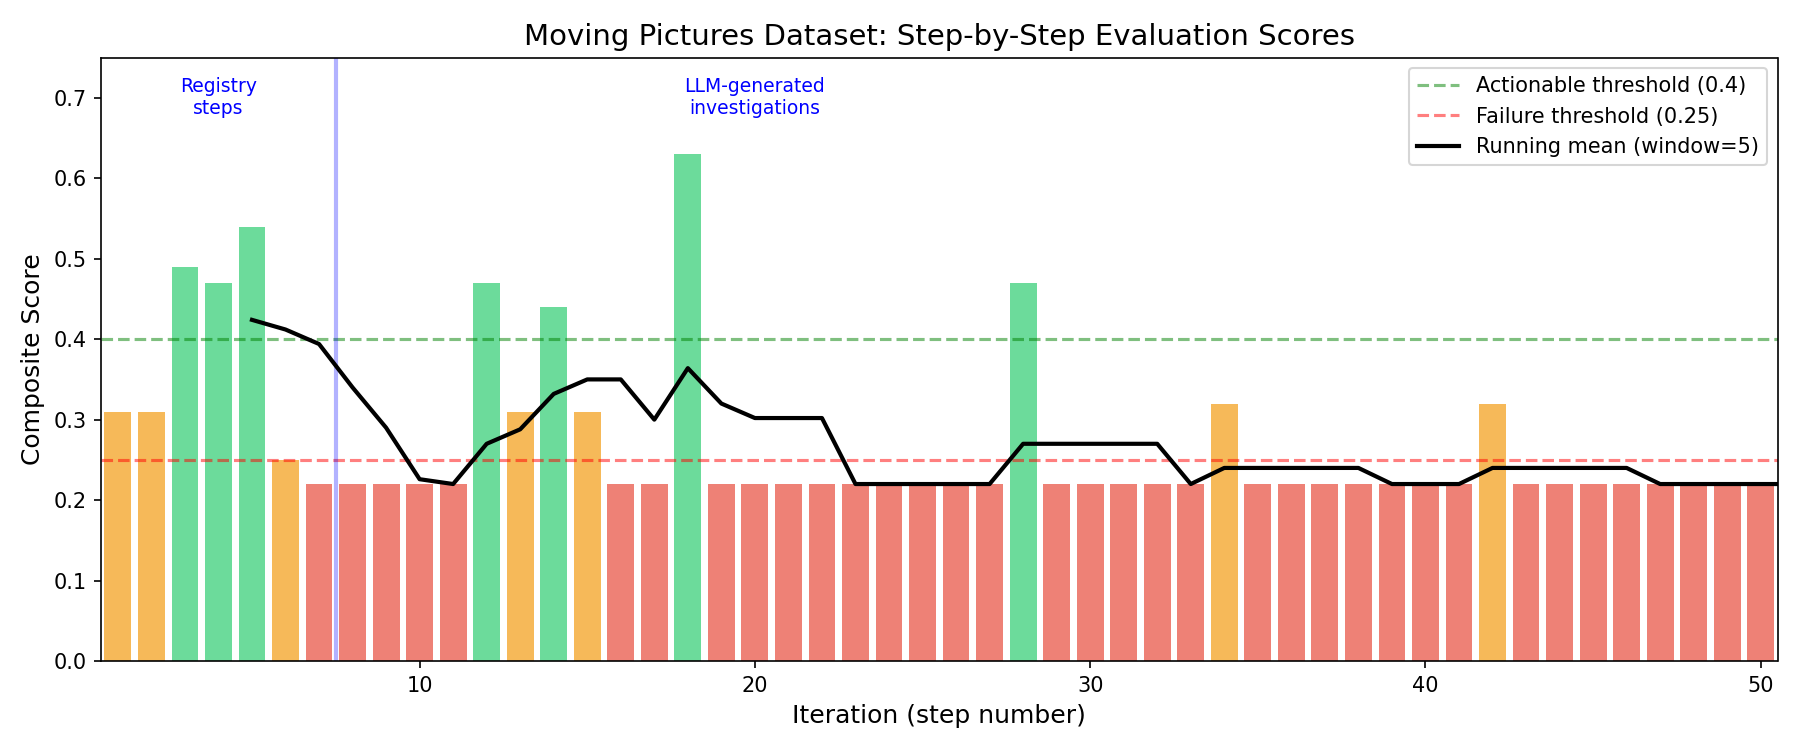
\includegraphics[width=\textwidth]{fig_convergence_scores.png}
\caption{Composite evaluation scores across iterations on the
Moving Pictures dataset.
Green bars: score $\geq 0.4$ (actionable);
orange: $0.25$--$0.4$;
red: $< 0.25$ (failed).
Blue vertical line separates registry steps (left) from
LLM-generated investigations (right).
Running mean (black line) shows declining trend as investigations
dominate.}
\label{fig:convergence}
\end{figure}

\paragraph{Critical finding: investigation loop.}
During execution, the LLM generated duplicate investigation titles
(e.g., ``Sparsity-aware analysis'' appeared $\sim$20 times).
This revealed a missing deduplication mechanism, which was subsequently
fixed by adding title-based duplicate checking and a maximum
investigation cap ($N = 8$).
This is an example of the system's closed-loop nature exposing its
own failure modes during operation.

\subsection{Cross-Dataset Comparison}
\label{sec:eval-crossdataset}

Figure~\ref{fig:dataset-comparison} compares evaluation scores across
the two datasets.
The taxonomy and differential steps achieved the highest scores
($> 0.6$) in both datasets, driven by strong biological signals
(high fold changes, known taxa).
Beta diversity scores diverged: Moving Pictures scored 0.47
(significant PERMANOVA) while Gravity scored 0.27 (non-significant).
This divergence is a correct reflection of the underlying data.

\begin{figure}[t]
\centering
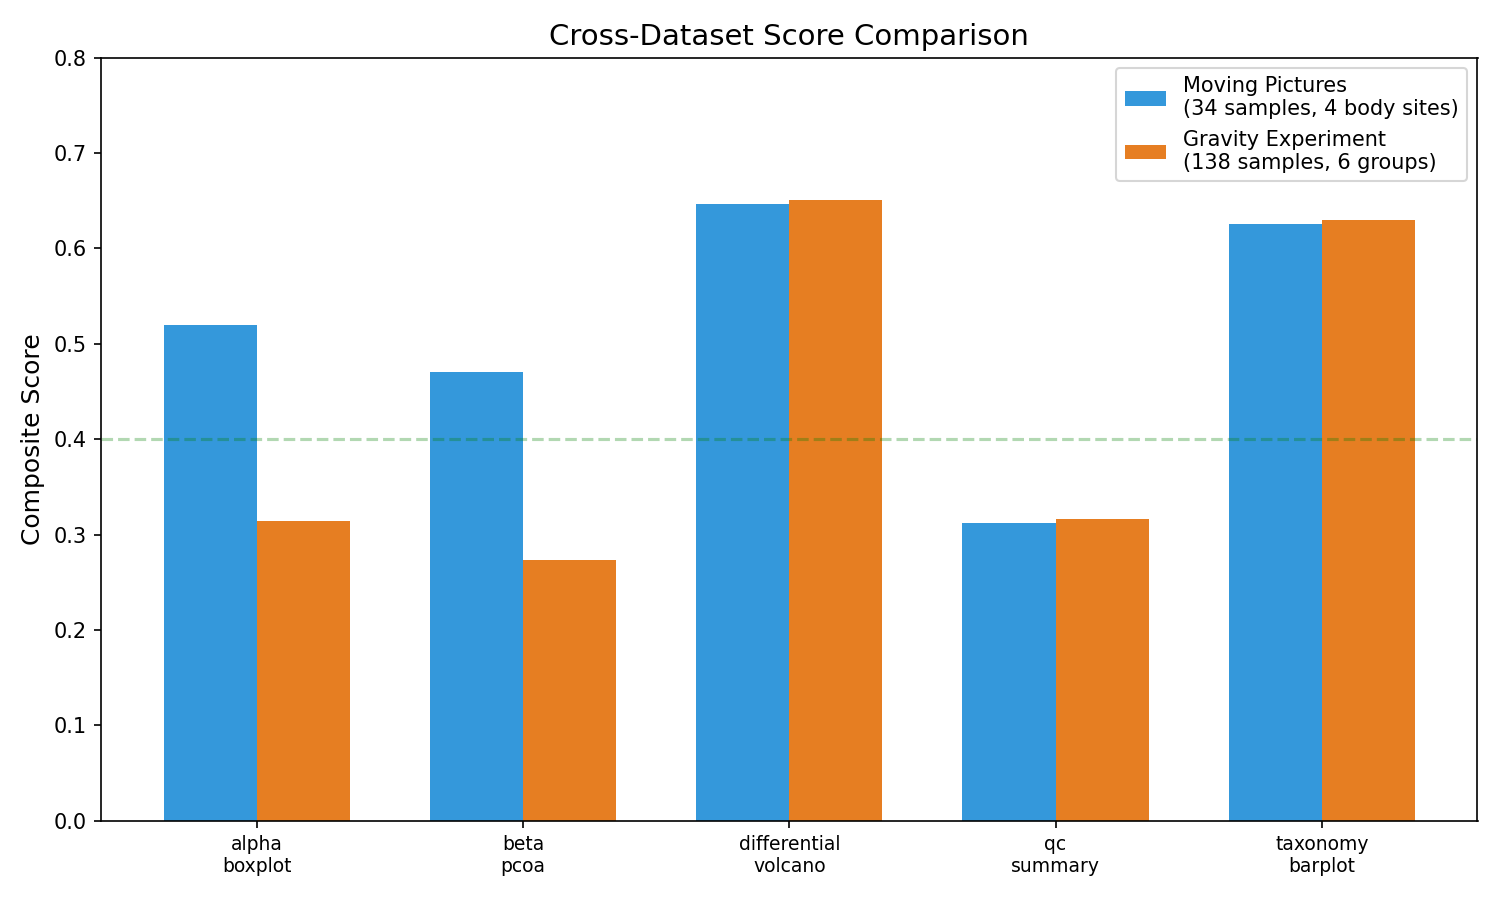
\includegraphics[width=\textwidth]{fig_dataset_comparison.png}
\caption{Composite scores for five analysis categories across two
datasets.
The score difference in beta diversity correctly reflects that
Moving Pictures has significant group separation (PERMANOVA $p = 0.005$)
while Gravity does not ($p = 0.81$).}
\label{fig:dataset-comparison}
\end{figure}

\begin{figure}[t]
\centering
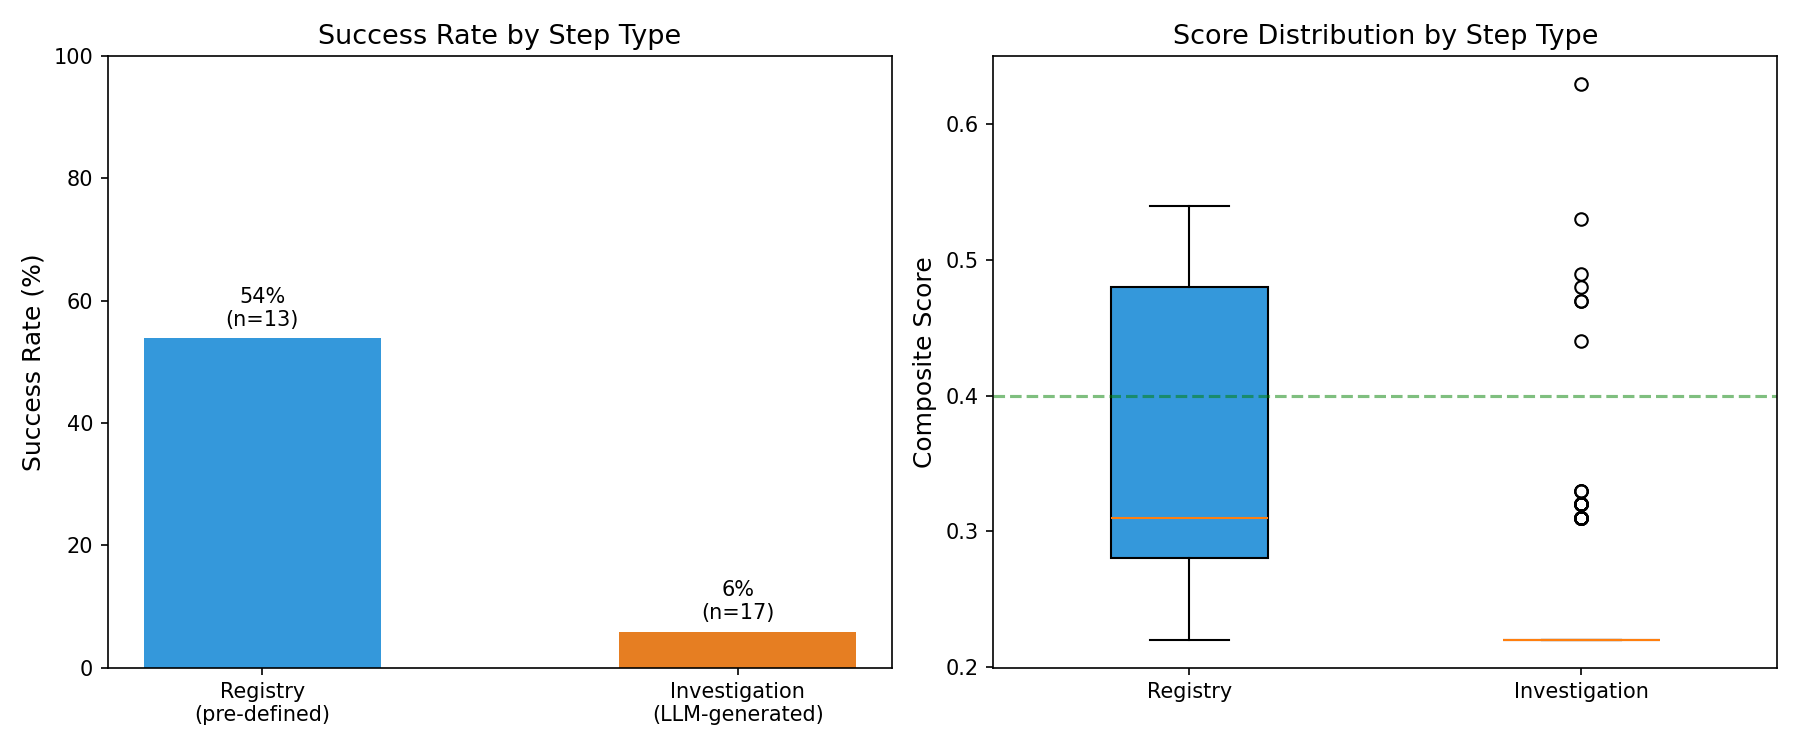
\includegraphics[width=\textwidth]{fig_error_distribution.png}
\caption{Left: success rate by step type.
Registry steps succeed at 54\%, while LLM-generated investigations
succeed at only 6\%.
Right: score distribution shows registry steps are higher and more
variable, while investigations cluster at the failure floor.}
\label{fig:error-types}
\end{figure}

\begin{figure}[t]
\centering
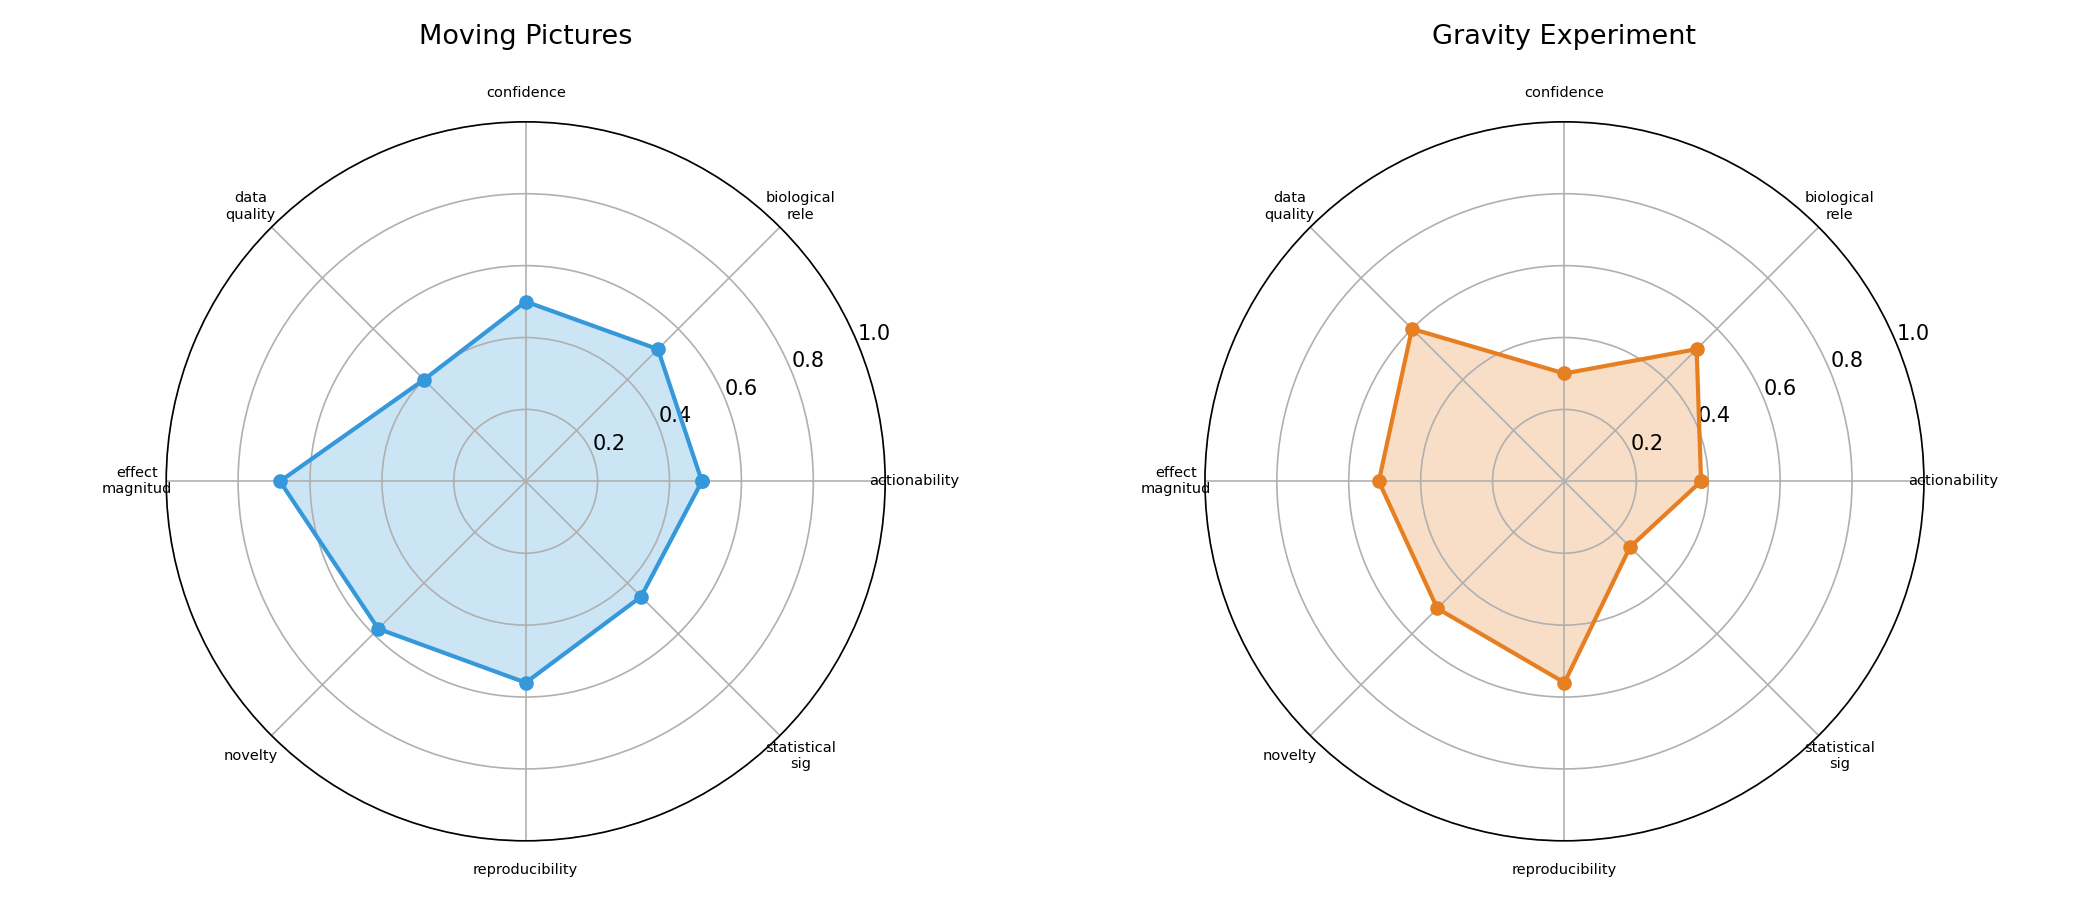
\includegraphics[width=\textwidth]{fig_radar_comparison.png}
\caption{Eight-axis radar plots comparing the average evaluation profile
across two datasets.
Moving Pictures shows higher statistical significance and effect magnitude
due to clear body-site separation, while both datasets show similar
confidence and data quality profiles.}
\label{fig:radar}
\end{figure}

% ======================================================================
\section{Limitations}
\label{sec:limits}
% ======================================================================

We identify the following limitations:

\begin{enumerate}
  \item \textbf{LLM dependence for code generation.}
    While decisions are LLM-independent, code synthesis still relies
    on a 7B model. Complex analyses (e.g., compositional regression)
    frequently fail even after 3 retries.
    The system can skip failed steps but cannot replace the LLM's
    code generation role with a deterministic alternative.

  \item \textbf{Statistical test approximations.}
    The pure-Python implementations use normal and $\chi^2$ approximations
    that are less accurate than exact tests for small samples ($n < 20$).
    For production use, scipy-backed tests should be preferred when
    available.

  \item \textbf{Fixed decision tree thresholds.}
    The thresholds (e.g., $p < 0.05$, effect $> 0.5$, fold change $> 5$)
    are drawn from literature conventions, not optimized for any
    particular dataset.
    Different research contexts may warrant different thresholds.

  \item \textbf{Eight-axis weights.}
    The default weights are hand-selected based on domain intuition.
    No learning or cross-validation was performed to optimize them.
    The experiment-type adjustment (e.g., increasing biological\_relevance
    for antibiotic studies) is also heuristic.

  \item \textbf{Single-omics scope.}
    The current implementation targets 16S rRNA amplicon sequencing only.
    Shotgun metagenomics, metatranscriptomics, and multi-omics
    integration are not supported.

  \item \textbf{Investigation generation quality.}
    LLM-generated investigation steps have a 6\% success rate,
    compared to 54\% for registry steps.
    The 7B model lacks sufficient capability for generating correct
    code for novel analysis tasks.
    Additionally, without deduplication, the LLM generates
    identical investigation titles repeatedly, requiring explicit
    caps and title-based filtering.

  \item \textbf{Limited evaluation scope.}
    The current evaluation covers two datasets.
    A comprehensive evaluation would require 5+ publicly available
    datasets spanning different experimental designs (paired,
    longitudinal, case-control) and a formal comparison with
    expert-curated analysis plans.
\end{enumerate}

% ======================================================================
\section{Discussion}
\label{sec:discussion}
% ======================================================================

\paragraph{Toward autonomous scientific analysis.}
\seqpipe\ takes a step toward systems that reason about data rather
than merely processing it.
The separation of evaluation (deterministic) from generation
(LLM-assisted) provides a template for similar systems in other
domains: any field where analysis proceeds iteratively---genomics,
proteomics, clinical trials---could benefit from a decision engine
that encodes domain heuristics as auditable, deterministic rules.

\paragraph{Implications for microbiome research.}
The practical impact is reduction of two failure modes:
(1)~\emph{over-analysis} (running beta dispersion when PERMANOVA is
non-significant) and (2)~\emph{under-analysis} (missing a follow-up
when an unexpected taxon enrichment is detected).
In our gravity experiment case study (138 samples, 6 groups),
the decision engine skipped 4 unnecessary beta analyses and added
5 targeted follow-ups, a workflow that an experienced analyst would
recognize as appropriate.

\paragraph{Space biology and real-time applications.}
The LLM-failure tolerance and deterministic decision layer make
\seqpipe\ suitable for environments where cloud connectivity is
unavailable---for example, microbiome monitoring on the International
Space Station, where data must be analyzed locally with limited
computational resources and no internet access.

\paragraph{Reproducibility as a design principle.}
By making the decision layer deterministic, \seqpipe\ ensures that
the analytical workflow is reproducible even when the LLM introduces
stochasticity in code generation.
Two runs on the same data will always make the same skip/add decisions,
even if the generated Python code differs syntactically.
This is a stronger reproducibility guarantee than any purely
LLM-driven system can provide.

% ======================================================================
\section{Conclusion}
\label{sec:conclusion}
% ======================================================================

We presented \seqpipe, a closed-loop system for adaptive microbiome
analysis that separates data inspection, quantitative evaluation,
deterministic decision-making, and LLM-assisted code generation
into distinct, composable layers.
The system reproduces the iterative reasoning loop of a human
bioinformatician: interpret results, update hypotheses, and
adapt the analysis plan---without requiring cloud connectivity
or expert intervention.

The central design principle is that \textbf{analytical decisions
should be grounded in data, not in language model outputs}.
Layer~1 reads data directly; Layer~2 decides deterministically;
Layer~3 generates code but does not override decisions.
This hierarchy yields a system that is auditable (every decision
has a traceable rule), reproducible (same data, same decisions),
and robust (LLM failure does not halt execution).

Our evaluation on two public datasets demonstrates that the
DecisionEngine correctly differentiates between datasets with
significant group separation (Moving Pictures: all beta follow-ups added)
and those without (Gravity: 4 beta steps skipped),
while the LLM-generated investigation layer reveals the current
limitations of 7B-parameter models for autonomous code generation
(6\% success rate).

We argue that interpretation-driven adaptive systems represent a
necessary evolution beyond static pipelines, and that the separation
of deterministic reasoning from stochastic generation is the key
architectural principle enabling this evolution.

% ======================================================================
% Bibliography
% ======================================================================

\bibliographystyle{plainnat}

\begin{thebibliography}{20}

\bibitem[Anderson(2001)]{anderson2001}
Anderson, M.~J. (2001).
A new method for non-parametric multivariate analysis of variance.
\textit{Austral Ecology}, 26(1), 32--46.

\bibitem[Bolyen et~al.(2019)]{qiime2}
Bolyen, E., et~al. (2019).
Reproducible, interactive, scalable and extensible microbiome data
science using QIIME 2.
\textit{Nature Biotechnology}, 37(8), 852--857.

\bibitem[Callahan et~al.(2016)]{callahan2016}
Callahan, B.~J., et~al. (2016).
DADA2: High-resolution sample inference from Illumina amplicon data.
\textit{Nature Methods}, 13(7), 581--583.

\bibitem[Di~Tommaso et~al.(2017)]{nextflow}
Di~Tommaso, P., et~al. (2017).
Nextflow enables reproducible computational workflows.
\textit{Nature Biotechnology}, 35(4), 316--319.

\bibitem[Feurer et~al.(2015)]{autosklearn}
Feurer, M., et~al. (2015).
Efficient and robust automated machine learning.
\textit{Advances in Neural Information Processing Systems}, 28.

\bibitem[Gloor et~al.(2017)]{gloor2017}
Gloor, G.~B., et~al. (2017).
Microbiome datasets are compositional: and this is not optional.
\textit{Frontiers in Microbiology}, 8, 2224.

\bibitem[Hong et~al.(2024)]{hong2024data}
Hong, S., et~al. (2024).
Data Interpreter: An LLM Agent For Data Science.
\textit{arXiv preprint arXiv:2402.18679}.

\bibitem[K{\"o}ster \& Rahmann(2012)]{snakemake}
K{\"o}ster, J. \& Rahmann, S. (2012).
Snakemake---a scalable bioinformatics workflow engine.
\textit{Bioinformatics}, 28(19), 2520--2522.

\bibitem[McMurdie \& Holmes(2014)]{mcmurdie2014}
McMurdie, P.~J. \& Holmes, S. (2014).
Waste not, want not: why rarefying microbiome data is inadmissible.
\textit{PLOS Computational Biology}, 10(4), e1003531.

\bibitem[Kothari et~al.(2019)]{autoweka}
Thornton, C., et~al. (2013).
Auto-WEKA: Combined selection and hyperparameter optimization of
classification algorithms.
\textit{KDD '13}, 847--855.

\bibitem[Wasserstein et~al.(2019)]{wasserstein2019}
Wasserstein, R.~L., et~al. (2019).
Moving to a world beyond ``$p < 0.05$''.
\textit{The American Statistician}, 73(sup1), 1--19.

\bibitem[Willis(2019)]{willis2019}
Willis, A.~D. (2019).
Rarefaction, alpha diversity, and statistics.
\textit{Frontiers in Microbiology}, 10, 2407.

\bibitem[Wilson \& Hilferty(1931)]{wilson1931}
Wilson, E.~B. \& Hilferty, M.~M. (1931).
The distribution of chi-square.
\textit{Proceedings of the National Academy of Sciences}, 17(12), 684--688.

\end{thebibliography}

\end{document}
